\chapter{Análisis, diseño e implementación del prototipo}
\label{ch:analisis-diseno-implementacion}

Este capítulo recoge el paso desde la idea general del teclado unimano hasta el prototipo desarrollado. Aquí el foco se pone en las decisiones técnicas: qué debe cumplir el sistema, con qué componentes se ha planteado, cómo se organiza la escritura y cómo se ha implementado el firmware.

El capítulo se estructura en cinco partes. Primero se definen los requisitos y restricciones del prototipo. Después se presentan los materiales y herramientas utilizados. A continuación se describe la arquitectura general del sistema, el diseño del método de escritura y la implementación hardware y software.

\section{Requisitos del sistema}
\label{sec:requisitos-sistema}

Los requisitos se han definido a partir del objetivo principal del proyecto: construir un dispositivo de entrada de texto pequeño, físico, silencioso y utilizable con una sola mano. No se pretende cubrir todos los posibles casos de accesibilidad, sino acotar un primer prototipo que pueda probar la viabilidad de la idea.
\clearpage
\subsection{Requisitos funcionales}
\label{subsec:requisitos-funcionales-nuevo}

 La Tabla~\ref{tab:requisitos-funcionales} recoge los requisitos considerados para el prototipo.

\begin{table}[H]
    \centering
    \caption{Requisitos funcionales del prototipo}
    \label{tab:requisitos-funcionales}
    \begin{tabularx}{\textwidth}{@{}p{0.16\textwidth}X@{}}
        \toprule
        \textbf{Código} & \textbf{Descripción} \\
        \midrule
        RF-01 & El dispositivo debe poder conectarse de forma inalámbrica a un ordenador, teléfono móvil o tableta. \\
        RF-02 & El sistema receptor debe reconocer el dispositivo como un teclado estándar. \\
        RF-03 & El joystick debe permitir distinguir ocho direcciones de entrada. \\
        RF-04 & Cada dirección del joystick debe asociarse a un carácter o acción según la capa activa. \\
        RF-05 & Los dos botones deben permitir seleccionar las capas disponibles. \\
        RF-06 & El teclado principal debe permitir introducir las letras del alfabeto. \\
        RF-07 & El sistema debe permitir introducir mayúsculas y acciones básicas como espacio, borrado e Intro. \\
        RF-08 & El dispositivo debe permitir acceder a un banco secundario de números, signos de puntuación y caracteres especiales. \\
        RF-09 & La matriz RGB debe mostrar información visual sobre el carácter seleccionado y la capa activa. \\
        RF-10 & El sistema debe incluir un modo de exploración que permita consultar caracteres sin enviarlos al dispositivo conectado. \\
        \bottomrule
    \end{tabularx}
\end{table}
\clearpage
\subsection{Requisitos no funcionales}
\label{subsec:requisitos-no-funcionales-nuevo}

Estos requisitos se resumen en la Tabla~\ref{tab:requisitos-no-funcionales}.

\begin{table}[H]
    \centering
    \caption{Requisitos no funcionales del prototipo}
    \label{tab:requisitos-no-funcionales}
    \begin{tabularx}{\textwidth}{@{}p{0.16\textwidth}X@{}}
        \toprule
        \textbf{Código} & \textbf{Descripción} \\
        \midrule
        RNF-01 & El dispositivo debe tener un tamaño suficientemente reducido para poder sostenerse en la palma de una mano. \\
        RNF-02 & La interacción principal debe poder realizarse con una sola mano y, preferiblemente, con tres dedos. \\
        RNF-03 & El uso del dispositivo debe ser silencioso para permitir su utilización en espacios compartidos. \\
        RNF-04 & El prototipo debe ser ligero y fácil de transportar. \\
        RNF-05 & Los controles deben poder distinguirse mediante el tacto. \\
        RNF-06 & El coste de los componentes debe mantenerse reducido. \\
        RNF-07 & La respuesta del sistema debe ser suficientemente rápida para no interrumpir la escritura. \\
        RNF-08 & El funcionamiento básico debe poder aprenderse sin conocimientos técnicos previos. \\
        \bottomrule
    \end{tabularx}
\end{table}

\subsection{Restricciones del proyecto}
\label{subsec:restricciones-nuevo}

Las restricciones del proyecto vienen marcadas por el tamaño, el coste, la disponibilidad de componentes y el alcance de un Trabajo de Fin de Grado. La Tabla~\ref{tab:restricciones-proyecto} recoge las principales restricciones consideradas durante el desarrollo.

\begin{table}[H]
    \centering
    \caption{Restricciones consideradas durante el desarrollo}
    \label{tab:restricciones-proyecto}
    \begin{tabularx}{\textwidth}{@{}p{0.24\textwidth}X@{}}
        \toprule
        \textbf{Restricción} & \textbf{Implicación en el diseño} \\
        \midrule
        Tamaño reducido & Limita la batería, la colocación de la matriz, el cableado y la forma de la carcasa. \\
        Bajo coste & Favorece el uso de componentes comunes, como joystick analógico, botones y microcontrolador compacto. \\
        Alimentación portátil & Obliga a considerar batería, carga, consumo de la matriz RGB y espacio interior. \\
        Compatibilidad & El dispositivo debe comportarse como teclado HID para evitar depender de una aplicación específica. \\
        Fabricación propia & La carcasa se plantea mediante modelado 3D e impresión 3D, lo que condiciona tolerancias, encajes y acabado. \\
        Alcance del prototipo & No se incluyen fabricación industrial, certificación comercial ni validación clínica con usuarios. \\
        \bottomrule
    \end{tabularx}
\end{table}

Como se muestra en la Figura~\ref{fig:componentes-principales}, los componentes electrónicos principales del prototipo son el microcontrolador, el joystick, la matriz RGB y el módulo de alimentación.

\begin{figure}[H]
    \centering

    \begin{subfigure}[t]{0.45\textwidth}
        \centering
        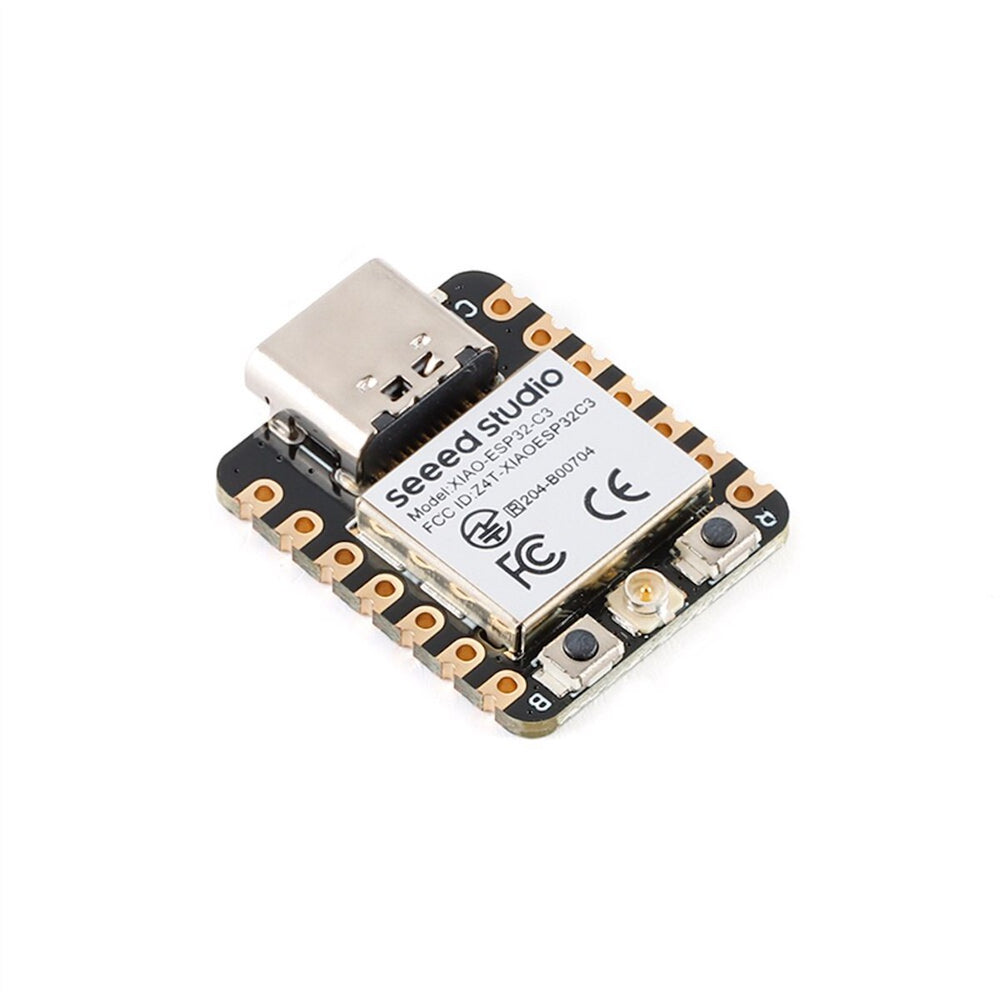
\includegraphics[width=\textwidth]{figures/xiao-esp32c3.png}
        \caption{Seeed Studio XIAO ESP32C3.}
        \label{fig:xiao-esp32c3}
    \end{subfigure}
    \hfill
    \begin{subfigure}[t]{0.45\textwidth}
        \centering
        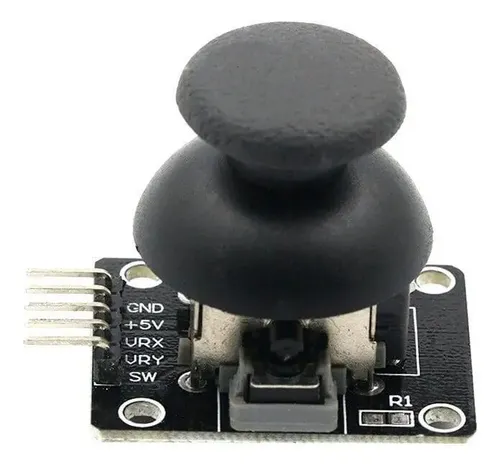
\includegraphics[width=\textwidth]{figures/joystick-hw504.png}
        \caption{Joystick HW-504.}
        \label{fig:joystick-hw504}
    \end{subfigure}

    \vspace{0.6cm}

    \begin{subfigure}[t]{0.45\textwidth}
        \centering
        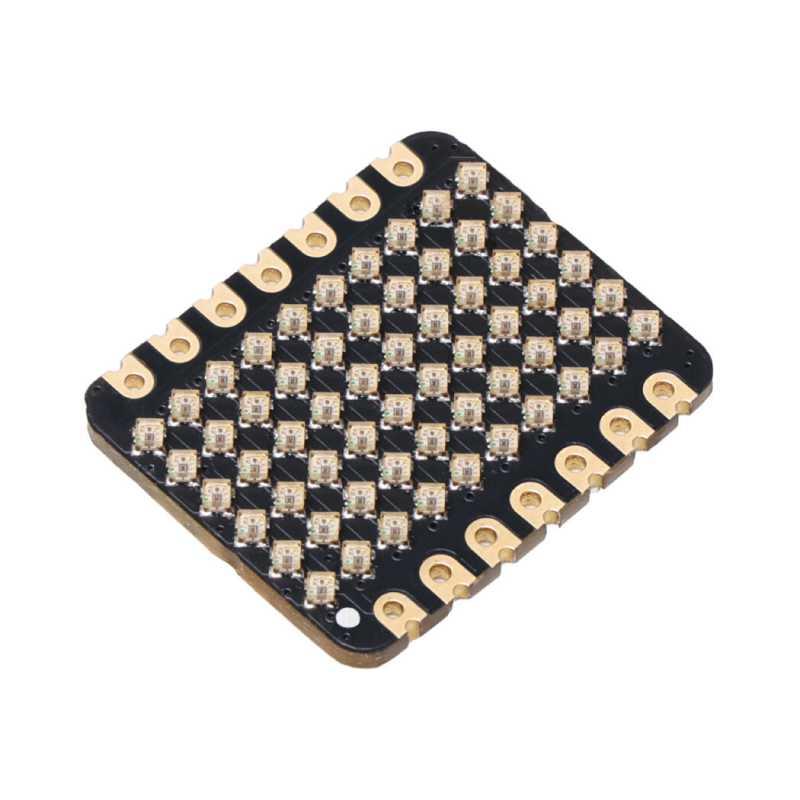
\includegraphics[width=\textwidth]{figures/matriz-rgb-6x10.png}
        \caption{Matriz RGB de \(6 \times 10\) para XIAO.}
        \label{fig:matriz-rgb}
    \end{subfigure}
    \hfill
    \begin{subfigure}[t]{0.45\textwidth}
        \centering
        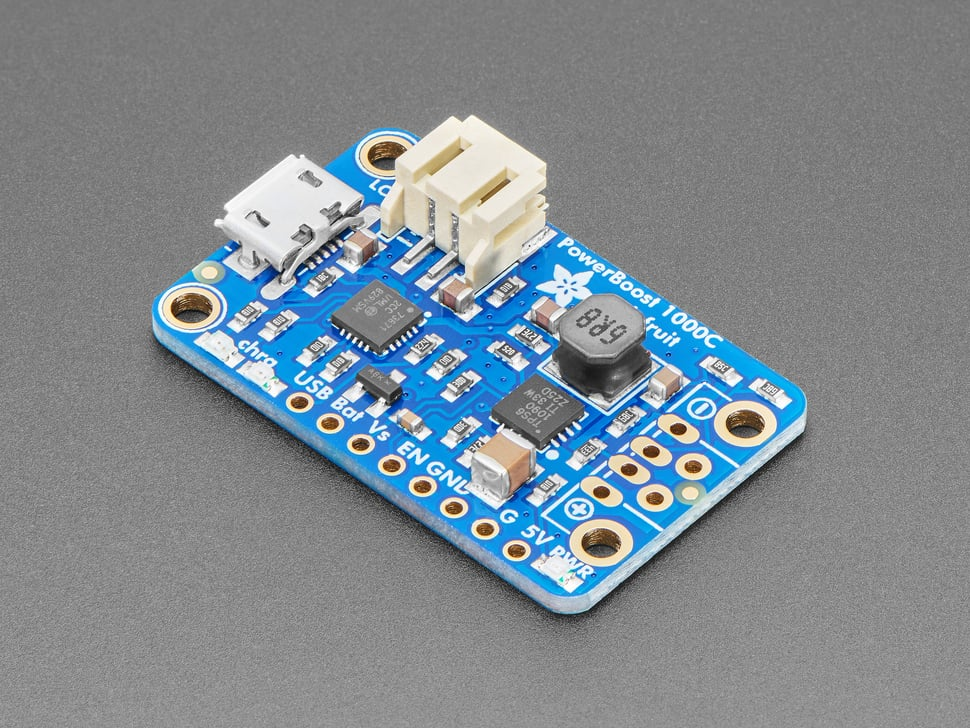
\includegraphics[width=\textwidth]{figures/powerboost-1000c.png}
        \caption{Módulo PowerBoost 1000C.}
        \label{fig:powerboost}
    \end{subfigure}

    \caption{Componentes electrónicos principales utilizados en el prototipo.}
    \label{fig:componentes-principales}
\end{figure}
\subsection{Criterios de diseño derivados}
\label{subsec:criterios-diseno}

A partir de los requisitos anteriores se fijaron varios criterios prácticos para guiar el diseño. El primero fue reducir al mínimo el número de controles físicos, por lo que se descartó una distribución basada en muchas teclas. El segundo fue mantener compatibilidad con dispositivos existentes, lo que llevó a utilizar Bluetooth HID. El tercero fue incluir una realimentación visual sencilla, ya que un sistema por capas puede ser difícil de aprender si el usuario no recibe información sobre el carácter seleccionado.

Estos criterios no sustituyen a los requisitos, sino que ayudan a convertirlos en decisiones concretas de diseño: joystick de ocho direcciones, dos botones para capas, matriz RGB para mostrar la selección y microcontrolador con conectividad Bluetooth.

\section{Materiales y herramientas}
\label{sec:materiales-herramientas}

Para el desarrollo del prototipo se utilizaron componentes electrónicos de pequeño tamaño y herramientas de desarrollo compatibles con ESP32. La Tabla~\ref{tab:materiales-herramientas} resume los elementos principales.

\begin{table}[H]
    \centering
    \caption{Materiales y herramientas utilizados}
    \label{tab:materiales-herramientas}
    \begin{tabularx}{\textwidth}{@{}p{0.30\textwidth}X@{}}
        \toprule
        \textbf{Elemento} & \textbf{Uso dentro del proyecto} \\
        \midrule
        Seeed Studio XIAO ESP32C3 & Microcontrolador principal, lectura de entradas, control de matriz y comunicación BLE HID \cite{xiaoESP32C3}. \\
        Joystick HW-504 & Entrada direccional principal, con dos ejes analógicos y pulsador integrado. \\
        Dos botones externos & Selección de capas mediante combinaciones de pulsación. \\
        Matriz RGB de \(6 \times 10\) para XIAO & Visualización del carácter seleccionado y de la capa activa \cite{seeedRGBMatrix}. \\
        PowerBoost 1000C & Gestión de alimentación portátil y elevación de tensión para alimentar la matriz RGB \cite{adafruitPowerBoost1000C}. \\
        ESP-IDF & Entorno de desarrollo para el firmware del ESP32C3. \\
        NimBLE & Pila Bluetooth utilizada para implementar el funcionamiento como teclado HID \cite{espressifNimBLE}. \\
        FreeCAD & Herramienta utilizada para el diseño de la carcasa. \\
        Voxelab Aquila X2 & Impresora 3D para fabricar la carcasa del prototipo. \\
        \bottomrule
    \end{tabularx}
\end{table}

La elección de estos componentes busca mantener el prototipo dentro de un tamaño razonable. La placa XIAO ESP32C3 permite integrar entradas analógicas, entradas digitales y comunicación Bluetooth en una placa compacta. La matriz RGB se utiliza como apoyo visual durante el aprendizaje, mientras que el joystick y los botones concentran la interacción física.

\section{Arquitectura general del sistema}
\label{sec:arquitectura-general-nuevo}

La arquitectura del prototipo se organiza alrededor del XIAO ESP32C3. Los controles físicos generan las entradas, el microcontrolador las interpreta y el resultado se envía al dispositivo receptor como una pulsación de teclado. Además, la matriz RGB ofrece información visual al usuario. La Figura~\ref{fig:arquitectura-general-sistema} muestra esta organización general.

\begin{figure}[H]
    \centering
    \begin{tikzpicture}[
        font=\small,
        bloque/.style={
            draw,
            rounded corners,
            thick,
            minimum width=3.0cm,
            minimum height=1.1cm,
            align=center
        },
        entrada/.style={bloque, fill=blue!8},
        proceso/.style={bloque, fill=gray!10},
        salida/.style={bloque, fill=green!10},
        energia/.style={bloque, fill=orange!15},
        flecha/.style={-Latex, thick},
        flechaenergia/.style={-Latex, thick, dashed}
    ]

        % Bloques principales
        \node[entrada] (controles) at (0,0) {Joystick\\y botones};
        \node[proceso] (mcu) at (4,0) {XIAO ESP32C3\\procesamiento};
        \node[salida] (hid) at (8,0) {Bluetooth HID\\teclado};
        \node[salida] (receptor) at (12,0) {Ordenador, móvil\\o tableta};

        % Realimentación visual
        \node[salida] (matriz) at (4,-2.6) {Matriz RGB\\realimentación visual};

        % Alimentación
        \node[energia] (alimentacion) at (4,2.4) {Batería y módulo\\de alimentación};

        % Flujo principal de datos
        \draw[flecha] (controles.east) -- (mcu.west);
        \draw[flecha] (mcu.east) -- (hid.west);
        \draw[flecha] (hid.east) -- (receptor.west);

        % Realimentación visual
        \draw[flecha] (mcu.south) -- (matriz.north);

        % Alimentación
        \draw[flechaenergia] (alimentacion.south) -- (mcu.north);
        \draw[flechaenergia]
            (alimentacion.east) -- ++(0.8,0)
            |- (matriz.east);

    \end{tikzpicture}
    \caption{Arquitectura general del sistema propuesto.}
    \label{fig:arquitectura-general-sistema}
\end{figure}En esta arquitectura, el ordenador no necesita conocer cómo se organizan las capas ni cómo se interpreta el joystick. Esa lógica queda dentro del firmware. El equipo receptor solo recibe eventos de teclado estándar, lo que simplifica el uso del prototipo en distintos dispositivos compatibles con teclados Bluetooth.

\section{Diseño del sistema de escritura}
\label{sec:diseno-escritura-nuevo}

El sistema de escritura se basa en combinar ocho direcciones del joystick con varias capas de caracteres. Esta organización permite obtener más entradas que controles físicos, sin convertir el dispositivo en un teclado completo.

\subsection{Direcciones del joystick}
\label{subsec:direcciones-joystick-nuevo}

El joystick entrega dos señales analógicas: una para el eje horizontal y otra para el eje vertical. A partir de esas lecturas se distinguen ocho direcciones y una posición central. La posición central no escribe ningún carácter; se utiliza como estado de reposo y como separación entre pulsaciones. La Figura~\ref{fig:ocho-direcciones-joystick} resume las direcciones utilizadas.

\begin{figure}[H]
    \centering
    \begin{tikzpicture}[
        font=\small,
        flecha/.style={-Latex, thick},
        limite/.style={densely dashed, gray!55},
        numero/.style={
            circle,
            draw,
            thick,
            fill=green!12,
            minimum size=0.62cm,
            inner sep=0pt,
            font=\bfseries\small
        },
        etiqueta/.style={
            font=\scriptsize,
            align=center,
            text width=2.1cm
        }
    ]

        \coordinate (c) at (0,0);

        \def\rExterior{2.55}
        \def\rMuerta{0.65}
        \def\rNumero{3.10}
        \def\rEtiqueta{4.25}

        % Círculo exterior
        \draw[thick] (c) circle (\rExterior);

        % Límites entre zonas
        \foreach \ang in {22.5,67.5,112.5,157.5,202.5,247.5,292.5,337.5} {
            \draw[limite] (\ang:\rMuerta) -- (\ang:\rExterior);
        }

        % Zona muerta central
        \fill[blue!10] (c) circle (\rMuerta);
        \draw[thick] (c) circle (\rMuerta);
        \node[align=center, font=\scriptsize] at (c) {zona\\muerta};

        % Direcciones
        \foreach \ang/\num/\txt in {
            90/0/{Arriba},
            45/1/{Arriba\\derecha},
            0/2/{Derecha},
            -45/3/{Abajo\\derecha},
            -90/4/{Abajo},
            -135/5/{Abajo\\izquierda},
            180/6/{Izquierda},
            135/7/{Arriba\\izquierda}
        } {
            \draw[flecha] (\ang:0.85) -- (\ang:2.05);
            \node[numero] at (\ang:\rNumero) {\num};
            \node[etiqueta] at (\ang:\rEtiqueta) {\txt};
        }

    \end{tikzpicture}
    \caption{Codificación de las ocho direcciones del joystick y zona muerta central.}
    \label{fig:ocho-direcciones-joystick}
\end{figure}

En el firmware se define una zona muerta alrededor del centro. Mientras las lecturas permanezcan dentro de esa zona, el sistema considera que el joystick está en reposo. Esta decisión reduce pulsaciones accidentales causadas por pequeñas variaciones mecánicas o eléctricas.

\subsection{Selección de capas mediante botones}
\label{subsec:capas-botones-nuevo}

Los dos botones se utilizan como selectores de capa. Cada botón puede estar pulsado o liberado, por lo que la combinación de ambos genera cuatro estados. El cálculo de la capa seleccionada por los botones se muestra en la Ecuación~\ref{eq:capa-botones}.

\begin{equation}
    C_{\text{botones}} = 2B_1 + B_2
    \label{eq:capa-botones}
\end{equation}

En la Ecuación~\ref{eq:capa-botones}, \(B_1\) y \(B_2\) representan el estado de los botones. Cada uno puede tomar el valor 0 o 1, y el resultado \(C_{\text{botones}}\) queda entre 0 y 3.

Además, el sistema dispone de dos bancos: un banco principal de letras y un banco secundario de números y símbolos. Para seleccionar el banco se utiliza un desplazamiento \(D_{\text{banco}}\), que puede valer 0 o 4. La capa real utilizada para consultar el carácter se calcula como se indica en la Ecuación~\ref{eq:capa-real}.

\begin{equation}
    C_{\text{real}} = C_{\text{botones}} + D_{\text{banco}}
    \label{eq:capa-real}
\end{equation}

El resultado de la Ecuación~\ref{eq:capa-real} siempre queda entre 0 y 7. Por tanto, el dispositivo puede trabajar con ocho capas en total sin añadir más botones físicos.

La Figura~\ref{fig:capas-teclado} muestra de forma esquemática cómo se combinan los dos botones con el cambio de banco.

\begin{figure}[H]
    \centering
    \resizebox{\textwidth}{!}{%
    \begin{tikzpicture}[
        font=\small,
        panel/.style={
            draw,
            rounded corners,
            thick
        },
        capa/.style={
            draw,
            rounded corners,
            thick,
            minimum width=2.35cm,
            minimum height=1.05cm,
            align=center
        },
        flecha/.style={-Latex, thick},
        flechacambio/.style={-Latex, thick, dashed}
    ]

        % Panel del banco principal
        \draw[panel, fill=blue!6] (-6.2,0.35) rectangle (6.2,3.25);
        \node[font=\bfseries] at (0,2.85)
            {Banco principal: letras y acciones frecuentes};
        \node[font=\scriptsize] at (0,2.48)
            {$D_{\text{banco}} = 0$};

        % Capas del banco principal
        \node[capa, fill=green!12] (c0) at (-4.5,1.45)
            {Capa 0\\{\scriptsize $B_1=0,\ B_2=0$}};
        \node[capa, fill=green!12] (c1) at (-1.5,1.45)
            {Capa 1\\{\scriptsize $B_1=0,\ B_2=1$}};
        \node[capa, fill=green!12] (c2) at (1.5,1.45)
            {Capa 2\\{\scriptsize $B_1=1,\ B_2=0$}};
        \node[capa, fill=green!12] (c3) at (4.5,1.45)
            {Capa 3\\{\scriptsize $B_1=1,\ B_2=1$}};

        % Panel del banco secundario
        \draw[panel, fill=orange!8] (-6.2,-3.25) rectangle (6.2,-0.35);
        \node[font=\bfseries] at (0,-0.75)
            {Banco secundario: números, puntuación y símbolos};
        \node[font=\scriptsize] at (0,-1.12)
            {$D_{\text{banco}} = 4$};

        % Capas del banco secundario
        \node[capa, fill=orange!16] (c4) at (-4.5,-2.15)
            {Capa 4\\{\scriptsize $B_1=0,\ B_2=0$}};
        \node[capa, fill=orange!16] (c5) at (-1.5,-2.15)
            {Capa 5\\{\scriptsize $B_1=0,\ B_2=1$}};
        \node[capa, fill=orange!16] (c6) at (1.5,-2.15)
            {Capa 6\\{\scriptsize $B_1=1,\ B_2=0$}};
        \node[capa, fill=orange!16] (c7) at (4.5,-2.15)
            {Capa 7\\{\scriptsize $B_1=1,\ B_2=1$}};

        % Cambio de banco por la derecha
        \draw[flechacambio]
            (c3.east) -- ++(0.85,0)
            |- node[pos=0.28, right, align=left, font=\scriptsize]
                {posición especial\\cambio a banco\\secundario}
            (c7.east);

        % Vuelta al banco principal por el exterior izquierdo
\draw[flechacambio]
    (c7.south) -- ++(0,-0.45)
    -- ++(-10.4,0)
    -- ++(0,4.25)
    -- (c0.west);

\node[
    font=\scriptsize,
    align=right,
    text width=2.3cm
] at (-7.45,0.55)
{posición especial\\vuelta a banco\\principal};
            (c0.west);

        % Leyenda inferior
        \node[
            draw,
            rounded corners,
            fill=gray!6,
            align=center,
            font=\scriptsize,
            text width=11.6cm
        ] at (0,-4.05)
        {Los dos botones seleccionan una de las cuatro capas disponibles. El banco activo añade un desplazamiento: 0 para el banco principal y 4 para el banco secundario.};

    \end{tikzpicture}%
    }
    \caption{Organización del teclado por bancos y capas.}
    \label{fig:capas-teclado}
\end{figure}

\subsection{Distribución de caracteres}
\label{subsec:distribucion-caracteres-nuevo}

Cada capa contiene ocho posiciones, una por cada dirección del joystick. La Tabla~\ref{tab:capas-principales-nuevo} muestra la distribución del banco principal. Las primeras capas contienen letras frecuentes, mientras que la última incluye letras restantes y acciones habituales.

\begin{table}[H]
    \centering
    \caption{Distribución del banco principal de letras}
    \label{tab:capas-principales-nuevo}
    \resizebox{\textwidth}{!}{%
        \begin{tabular}{lcccccccc}
            \toprule
            \textbf{Capa} & \textbf{Arriba} & \textbf{Sup. dcha.} & \textbf{Derecha} & \textbf{Inf. dcha.} & \textbf{Abajo} & \textbf{Inf. izq.} & \textbf{Izquierda} & \textbf{Sup. izq.} \\
            \midrule
            0 & e & a & o & s & r & n & i & d \\
            1 & l & c & u & m & p & t & b & g \\
            2 & v & y & q & h & f & z & j & ñ \\
            3 & x & k & w & Intro & Borrar & Mayúsculas & Espacio & Banco secundario \\
            \bottomrule
        \end{tabular}%
    }
\end{table}

La Tabla~\ref{tab:capas-secundarias-nuevo} recoge el banco secundario, destinado a números, signos de puntuación y símbolos. Se mantiene la misma lógica de uso: botones para seleccionar capa y joystick para seleccionar posición.

\begin{table}[H]
    \centering
    \caption{Distribución del banco secundario de números y símbolos}
    \label{tab:capas-secundarias-nuevo}
    \resizebox{\textwidth}{!}{%
        \begin{tabular}{lcccccccc}
            \toprule
            \textbf{Capa} & \textbf{Arriba} & \textbf{Sup. dcha.} & \textbf{Derecha} & \textbf{Inf. dcha.} & \textbf{Abajo} & \textbf{Inf. izq.} & \textbf{Izquierda} & \textbf{Sup. izq.} \\
            \midrule
            4 & 0 & 1 & 2 & 3 & 4 & 5 & 6 & 7 \\
            5 & 8 & 9 & . & : & , & ; & - & \_ \\
            6 & ¿ & ? & ¡ & ! & `` & @ & ( & ) \\
            7 & = & + & * & \& & \textless & \textgreater & Espacio & Banco principal \\
            \bottomrule
        \end{tabular}%
    }
\end{table}

\section{Diseño e implementación hardware}
\label{sec:hardware-nuevo}

\subsection{Microcontrolador}
\label{subsec:microcontrolador-nuevo}

El microcontrolador elegido es el Seeed Studio XIAO ESP32C3. Su tamaño reducido facilita integrarlo en una carcasa de mano, y sus entradas permiten conectar los dos ejes analógicos del joystick, los dos botones, el pulsador integrado y la matriz RGB \cite{xiaoESP32C3}.

El uso de una placa con Bluetooth integrado evita añadir un módulo inalámbrico adicional. Esto simplifica el prototipo y reduce tanto el espacio ocupado como el número de conexiones internas.

\subsection{Joystick, botones y matriz RGB}
\label{subsec:joystick-botones-matriz-nuevo}

El joystick HW-504 se utiliza como entrada principal. Sus dos ejes se conectan a entradas ADC del microcontrolador. El pulsador integrado del joystick se reserva para funciones menos frecuentes, como alternar entre el modo de escritura y el modo de exploración.

Los dos botones externos se conectan a entradas digitales con resistencias internas de \textit{pull-up}. Así, cuando el botón no está pulsado la entrada queda en nivel alto, y al pulsarlo pasa a nivel bajo. Esta configuración reduce componentes externos y simplifica el montaje.

La matriz RGB de \(6 \times 10\) LEDs se controla mediante una única línea de datos. En el prototipo se utiliza para mostrar un carácter cada vez, junto con una indicación visual de la capa activa \cite{seeedRGBMatrix}. No se pretende que funcione como pantalla de texto completo, sino como apoyo durante la selección y el aprendizaje.

Las conexiones principales del prototipo se resumen en la Tabla~\ref{tab:conexiones-hardware-nuevo}.

\begin{table}[H]
    \centering
    \caption{Conexiones principales entre componentes y microcontrolador}
    \label{tab:conexiones-hardware-nuevo}
    \begin{tabularx}{\textwidth}{@{}p{0.24\textwidth}Xp{0.20\textwidth}@{}}
        \toprule
        \textbf{Componente} & \textbf{Señal} & \textbf{Pin} \\
        \midrule
        Joystick & Eje horizontal & GPIO 2 \\
        Joystick & Eje vertical & GPIO 3 \\
        Joystick & Pulsador integrado & GPIO 4 \\
        Botón 1 & Selección de capa & GPIO 5 \\
        Botón 2 & Selección de capa & GPIO 6 \\
        Matriz RGB & Línea de datos & GPIO 10 \\
        \bottomrule
    \end{tabularx}
\end{table}

\subsection{Alimentación}
\label{subsec:alimentacion-nuevo}

El sistema está pensado para funcionar con batería. La matriz RGB es el componente que más condiciona la alimentación, ya que requiere una tensión estable y puede consumir bastante más que el microcontrolador si se encienden muchos LEDs con brillo alto.

La Figura~\ref{fig:alimentacion-sistema} muestra el esquema de alimentación planteado. La batería alimenta el módulo PowerBoost 1000C, que proporciona una salida elevada para el microcontrolador y la matriz RGB. Todos los módulos comparten una referencia común de tierra.

\begin{figure}[H]
    \centering
    \resizebox{0.98\textwidth}{!}{%
    \begin{tikzpicture}[
        font=\small,
        bloque/.style={
            draw,
            rounded corners,
            thick,
            minimum width=3.1cm,
            minimum height=1.15cm,
            align=center
        },
        modulo/.style={bloque, fill=blue!8},
        alimentacion/.style={bloque, fill=orange!14},
        carga/.style={bloque, fill=green!10},
        flecha/.style={-Latex, thick},
        gnd/.style={thick, dashed},
        etiqueta/.style={font=\small, fill=white, inner sep=1.5pt}
    ]

        % -------------------------
        % Valores editables
        % -------------------------
        \def\xBat{-6.6}
        \def\xBoost{-1.9}
        \def\xXiao{3.2}
        \def\xJoy{8.2}

        \def\yCentro{0}
        \def\yXiao{1.45}
        \def\yMatriz{-1.10}
        \def\yGnd{-2.60}
        \def\yNota{-3.45}

        % -------------------------
        % Bloques
        % -------------------------
        \node[alimentacion] (bat) at (\xBat,\yCentro)
            {Batería\\LiPo 3,7 V};

        \node[alimentacion] (boost) at (\xBoost,\yCentro)
            {PowerBoost\\1000C};

        \node[modulo] (xiao) at (\xXiao,\yXiao)
            {XIAO\\ESP32C3};

        \node[carga] (matriz) at (\xXiao,\yMatriz)
            {Matriz RGB\\$6 \times 10$};

        \node[carga] (joy) at (\xJoy,\yXiao)
            {Joystick\\HW-504};

        % -------------------------
        % Alimentación positiva
        % -------------------------
        \draw[flecha]
            (bat.east) -- node[etiqueta, above] {3,7 V} (boost.west);

        \coordinate (salida5v) at (0.10,\yCentro);

        \draw[flecha]
            (boost.east) -- (salida5v);

        \draw[flecha]
            (salida5v) |- node[etiqueta, pos=0.72, above] {5 V} (xiao.west);

        \draw[flecha]
            (salida5v) |- node[etiqueta, pos=0.72, below] {5 V} (matriz.west);

        \draw[flecha]
            (xiao.east) -- node[etiqueta, above] {3,3 V} (joy.west);

        % -------------------------
        % Bus de GND común
        % -------------------------
        \draw[gnd] (-2.4,\yGnd) -- (6.6,\yGnd)
            node[etiqueta, right] {GND común};

        % PowerBoost: baja un poco, se desplaza a la izquierda y luego baja al bus
        \path (boost.south) ++(0,-0.45) coordinate (boostgnda);
        \path (boostgnda) ++(-0.85,0) coordinate (boostgndb);
        \draw[gnd]
            (boost.south) -- (boostgnda) -- (boostgndb) -- ({\xBoost-0.85},\yGnd);

        % Matriz y joystick: conexión directa al bus
        \draw[gnd] (matriz.south) -- (\xXiao,\yGnd);
        \draw[gnd] (joy.south) -- (\xJoy,\yGnd);

        % XIAO: baja un poco, se desplaza a la derecha y luego baja al bus sin tocar la matriz
        \draw[gnd]
        (xiao.south) -- ++(0,-0.30) -- ++(1.80,0) -- ({\xXiao+1.80},\yGnd);                     % -------------------------
        % Nota inferior
        % -------------------------
        \node[
            draw,
            rounded corners,
            fill=gray!6,
            align=center,
            font=\scriptsize,
            text width=10.8cm
        ] at (1.7,\yNota)
        {El PowerBoost proporciona la línea de 5 V para la XIAO y la matriz RGB. El joystick se alimenta desde la salida de 3,3 V de la XIAO para evitar aplicar 5 V a las entradas analógicas.};

    \end{tikzpicture}%
    }
    \caption{Esquema de alimentación del prototipo.}
    \label{fig:alimentacion-sistema}
\end{figure}

En la implementación se debe controlar el brillo de la matriz para reducir consumo y evitar picos de corriente innecesarios. Esta decisión se tendrá en cuenta también en el capítulo de pruebas, donde la autonomía y el consumo forman parte de los resultados a revisar.

\section{Diseño e implementación software}
\label{sec:software-nuevo}

El firmware se ha desarrollado en C con ESP-IDF. La implementación se divide en tareas: una parte lee el joystick, otra procesa los botones y las capas, otra actualiza la matriz RGB y otra gestiona el envío de informes HID por Bluetooth.

La Figura~\ref{fig:flujo-software} resume el flujo principal del programa desde que el usuario mueve el joystick hasta que se envía una tecla.

\begin{figure}[H]
    \centering
    \resizebox{\textwidth}{!}{%
    \begin{tikzpicture}[
        font=\small,
        bloque/.style={
            draw,
            rounded corners,
            thick,
            minimum width=2.75cm,
            minimum height=1.05cm,
            align=center,
            fill=blue!8
        },
        bloqueespera/.style={
            draw,
            rounded corners,
            thick,
            minimum width=2.75cm,
            minimum height=1.05cm,
            align=center,
            fill=gray!10
        },
        decision/.style={
            draw,
            diamond,
            thick,
            aspect=2.35,
            minimum width=2.50cm,
            minimum height=1.25cm,
            align=center,
            fill=yellow!20,
            inner sep=1pt
        },
        flecha/.style={-Latex, thick},
        etiqueta/.style={
            font=\scriptsize,
            fill=white,
            inner sep=1.2pt
        }
    ]

        % -------------------------
        % Fila superior
        % -------------------------
        \node[bloque] (adc) at (0,0)
            {Leer joystick\\ADC X/Y};

        \node[bloque] (dir) at (3.6,0)
            {Calcular\\dirección};

        \node[decision] (centro) at (7.0,0)
            {¿Centro?};

        \node[bloque] (capa) at (10.6,0)
            {Calcular\\capa real};

        \node[bloque] (tabla) at (14.3,0)
            {Consultar tabla\\de caracteres};

        % -------------------------
        % Fila inferior más separada
        % -------------------------
        \node[bloqueespera] (espera) at (2.4,-3.10)
            {Esperar nueva\\entrada};

        \node[bloque] (hid) at (6.5,-3.10)
            {Enviar pulso\\HID};

        \node[decision] (modo) at (10.7,-3.10)
    {¿Modo\\escritura?};

\node[bloque] (matriz) at (15.0,-3.10)
    {Mostrar carácter\\en matriz RGB};

        % -------------------------
        % Flujo principal
        % -------------------------
        \draw[flecha] (adc.east) -- (dir.west);
        \draw[flecha] (dir.east) -- (centro.west);

        \draw[flecha]
            (centro.east) -- node[etiqueta, above] {no} (capa.west);

        \draw[flecha] (capa.east) -- (tabla.west);

        \draw[flecha]
            (tabla.south) -- (matriz.north);

        \draw[flecha]
            (matriz.west) -- (modo.east);

        % -------------------------
        % Caso joystick en centro
        % -------------------------
        \draw[flecha]
            (centro.south) -- ++(0,-1.05)
            -| node[etiqueta, pos=0.22, right] {sí}
            (espera.north);

        % -------------------------
        % Decisión modo escritura
        % -------------------------
        \draw[flecha]
            (modo.west) -- node[etiqueta, above] {sí} (hid.east);

        \draw[flecha]
            (hid.west) -- (espera.east);

        \draw[flecha]
            (modo.south) -- ++(0,-0.95)
            -| node[etiqueta, pos=0.18, right] {no}
            (espera.south);

    \end{tikzpicture}%
    }
    \caption{Flujo principal del firmware durante la selección de caracteres.}
    \label{fig:flujo-software}
\end{figure}

\subsection{Lectura del joystick}
\label{subsec:lectura-joystick-nuevo}

Los dos ejes del joystick se leen con el controlador ADC en modo \textit{oneshot} \cite{espressifADCOneshot}. Cada lectura devuelve un valor numérico que depende de la posición física del joystick. En las pruebas iniciales se observaron valores centrales cercanos a 1995 y 1882, y extremos próximos a 0 y 4095.

La función de lectura compara esos valores con rangos establecidos para identificar una de las ocho direcciones. Si ambos ejes se mantienen dentro del margen definido alrededor del centro, la función devuelve el estado de reposo. Este reposo es importante porque evita que una misma inclinación genere caracteres repetidos de forma no deseada.

\subsection{Gestión de botones, capas y modos}
\label{subsec:gestion-botones-capas-nuevo}

Los botones se gestionan mediante interrupciones GPIO. La interrupción no procesa directamente la lógica de capas; solo introduce un evento en una cola de FreeRTOS. Después, una tarea lee el estado real de los controles y actualiza la capa activa.

Se introduce una espera breve antes de leer los botones para reducir el efecto del rebote mecánico y permitir que las pulsaciones simultáneas se detecten como una combinación. Este detalle es importante porque una diferencia de pocos milisegundos entre los dedos podría activar una capa incorrecta.

La combinación de los dos botones externos y el pulsador del joystick permite alternar entre modo de escritura y modo de exploración. En modo de escritura, el carácter seleccionado se envía por Bluetooth. En modo de exploración, el carácter solo se muestra en la matriz RGB.

\subsection{Selección, visualización y envío de caracteres}
\label{subsec:seleccion-visualizacion-envio-nuevo}

El firmware utiliza dos tablas de \(8 \times 8\). La primera contiene los códigos HID que se envían al dispositivo receptor. La segunda contiene la representación textual que se muestra en la matriz RGB.

Cuando se detecta una dirección válida, se calcula la capa real mediante la Ecuación~\ref{eq:capa-real}. Después se consulta la tabla correspondiente y se obtiene el carácter o acción asociada. Algunas posiciones no escriben directamente un carácter, sino que activan una acción interna, como cambiar al banco secundario.

Antes de enviar el carácter, el sistema lo muestra en la matriz RGB. La representación se realiza mediante una fuente de \(6 \times 10\) píxeles. Cada carácter ocupa diez bytes, uno por fila, y cada bit indica si el LED correspondiente debe encenderse. En el caso de caracteres como la \textit{ñ}, se ha añadido una conversión para tratar correctamente la codificación UTF-8.

Cuando el dispositivo está conectado y se encuentra en modo de escritura, el envío se realiza como una pulsación HID. Primero se envía un informe con la tecla pulsada y, después de una breve espera, se envía un informe vacío para indicar la liberación de la tecla. Esta separación evita que el sistema receptor interprete que la tecla se mantiene pulsada.

\subsection{Comunicación Bluetooth HID}
\label{subsec:bluetooth-hid-nuevo}

La comunicación inalámbrica se implementa mediante Bluetooth Low Energy y la pila NimBLE. El dispositivo se anuncia como un teclado y expone el servicio HID necesario para enviar informes de teclado al equipo receptor.

El informe utilizado sigue el formato habitual de teclado: un byte para modificadores, un byte reservado y seis posiciones para códigos de tecla. Esto permite enviar letras simples y también combinaciones con modificadores como \textit{Shift} o \textit{AltGr}. La compatibilidad con HID es una de las decisiones clave del proyecto, porque evita depender de una aplicación intermedia.

Una limitación práctica es que algunos símbolos dependen de la distribución de teclado configurada en el sistema operativo receptor. Por este motivo, las pruebas deben comprobar no solo que se envían informes HID, sino que los caracteres resultantes son los esperados en la distribución usada.

\section{Diseño físico e integración prevista}
\label{sec:diseno-fisico-integracion}

La carcasa se plantea como un elemento fundamental del prototipo, no solo como una protección externa. La posición del joystick, los botones y la matriz condiciona directamente la comodidad y la facilidad de uso.

El diseño se inspira en mandos de una sola mano. El joystick se sitúa en la zona superior para que pueda manejarse con el pulgar. Los botones se colocan en una posición alcanzable con el índice y el corazón. La matriz RGB debe quedar visible, pero sin obligar a girar la muñeca de forma incómoda.

La carcasa se diseña en FreeCAD y se plantea para impresión 3D. Esta decisión permite modificar la forma durante el desarrollo y realizar varias iteraciones si la primera versión no resulta cómoda. La integración final debe reservar espacio para el microcontrolador, la matriz, el sistema de alimentación, la batería y el cableado interno.

\section{Justificación de decisiones principales}
\label{sec:justificacion-decisiones-principales}

Las decisiones principales del prototipo se resumen en la Tabla~\ref{tab:justificacion-decisiones}. Se presenta esta información de forma concentrada para evitar repetir la explicación técnica desarrollada en las secciones anteriores.

\begin{table}[H]
    \centering
    \caption{Resumen de decisiones principales de diseño}
    \label{tab:justificacion-decisiones}
    \begin{tabularx}{\textwidth}{@{}p{0.28\textwidth}X@{}}
        \toprule
        \textbf{Decisión} & \textbf{Motivo} \\
        \midrule
        Joystick de ocho direcciones & Permite obtener varias selecciones con un único dedo y reduce el número de controles físicos. \\
        Dos botones para capas & Multiplican el número de caracteres disponibles sin añadir muchas teclas. \\
        Banco principal y banco secundario & Separa letras frecuentes de números y símbolos, manteniendo una lógica de uso consistente. \\
        Matriz RGB & Ayuda a visualizar la selección y reduce la dependencia de memoria durante el aprendizaje. \\
        Bluetooth HID & Permite que el prototipo se comporte como un teclado estándar sin aplicación intermedia. \\
        Impresión 3D & Facilita modificar la carcasa y adaptar la posición de los controles durante el desarrollo. \\
        \bottomrule
    \end{tabularx}
\end{table}

En conjunto, el diseño intenta equilibrar tres aspectos: reducir la interacción física, mantener compatibilidad con dispositivos reales y conservar margen para modificar la distribución durante futuras pruebas.
